%%%%%%%%%%%%%%%%%%%%%%%%%%%%%%%%%% Version: December, 20th 1998.
\documentclass{amsart}    % Specifies the document style.

\usepackage{amsmath}
\usepackage{fullpage}
\usepackage{tikz}
\usepackage{hyperref}
\usepackage{pgfplots}
\usepackage{pgfplotstable}

%\usepackage{refcheck}

\newcommand{\D}{\displaystyle}
\newcommand{\norm}[2]{\left\|#1\right\|_{#2}}

\newcommand{\red}[1]{{\color{red}#1}}


%\newcounter{equation}[section]
\renewcommand{\theequation}{\thesection.\arabic{equation}}

\newcommand{\N}{\mathbb{N}} 
\newcommand{\Z}{\mathbb{Z}}
\newcommand{\Q}{\mathbb{Q}}
\newcommand{\R}{\mathbb{R}} 
\newcommand{\C}{\mathbb{C}}

\newcommand{\arctg}{\mathop{\hbox{\rm arctg}}\nolimits}
\newcommand{\cotg}{\mathop{\hbox{\rm cotg}}\nolimits}
\newcommand{\tg}{\mathop{\hbox{\rm tg}}\nolimits}
\newcommand{\sen}{\mathop{\hbox{\rm sen}}\nolimits}
\newcommand{\Fin}{\begin{flushright} \rule{2mm}{2mm} \end{flushright}}
\newcommand{\Tan}{\mathop{\hbox{\rm tanh}}\nolimits}
\newcommand{\tin}{\mathop{\hbox{\rm tany}}\nolimits}
\newcommand{\Cos}{\mathop{\hbox{\rm cosh}}\nolimits}
\newcommand{\Sin}{\mathop{\hbox{\rm sinh}}\nolimits}
\newcommand{\Cot}{\mathop{\hbox{\rm coth}}\nolimits}
\newcommand{\sg}{\mathop{\hbox{\rm sgn}}\nolimits}
\newcommand{\lm}{\mathop{\hbox{\rm lim\,inf}}\limits}
\newcommand{\ssup}{\mathop{\hbox{\rm sup}}\limits}
%\newcommand{\grano}{\mathop{\hbox{\cal O}}\limits}
\newcommand{\arc}{\mathop{\hbox{\rm arc\,cos}}\nolimits}
\newcommand{\rightt}{\hbox{ \rule[-3mm]{0,1mm}{1cm} }}
\newcommand{\maxx}{\mathop{\hbox{\rm max}}\limits}
\newcommand{\spa}{\mathop{\hbox{\rm span}}\limits}
\newcommand{\ddiv}{\mathop{\hbox{\rm div}}\limits}
\newcommand{\Fn} {\rule{2mm}{2mm}}
\newcommand{\llaved}{\mathop{\hbox{ \Huge $]$}}\limits}
\newcommand{\itt}{\mathop{\hbox{\rm int}}\limits}
\newcommand{\intd}{\displaystyle\int \kern -7pt \int}

\newtheorem{definition}{\bf Definition}[section]
\newtheorem{theorem}{\bf Theorem}[section]
\newtheorem{remark}{\bf Remark}[section]
\newtheorem{proposition}{\bf Proposition}[section]
\newtheorem{corollary}{\bf Corollary}[section]
\newtheorem{lemma}{\bf Lemma}[section]


\date{}

\title{Null controllability of a nonlocal heat equation with integral kernel}

\author{Umberto Biccari\textsuperscript{1,2}}  
\address{\textsuperscript{1}\,DeustoTech, University of Deusto, 48007 Bilbao, Basque Country, Spain.}
\address{\textsuperscript{2}\,Facultad de Ingenier\'ia, Universidad de Deusto, Avenida de las Universidades 24, 48007 Bilbao, Basque Country, Spain, +34 944139003 - 3282.}
\email{umberto.biccari@deusto.es, u.biccari@gmail.com, victor.santamaria@deusto.es}
\thanks{The work of Umberto Biccari was partially supported by the Advanced Grant DYCON (Dynamic Control) of the European Research Council Executive Agency, by the MTM2014-52347 Grant of the MINECO (Spain) and by the Air Force Office of Scientific Research under the Award No: FA9550-15-1-0027.} 

\author{V\'ictor Hern\'andez-Santamar\'ia\textsuperscript{1,2}}
\thanks{The work of V\'ictor Hern\'andez-Santamar\'ia was partially supported by the
	Advanced Grant DYCON (Dynamic Control) of the European Research Council Executive Agency.} 

\keywords{Null controllability, heat equation, nonlocal terms, Carleman inequalities}

\subjclass[2010]{93B05, 93B07, 93C20}

\begin{document}           

\maketitle

\begin{abstract}
We consider a linear nonlocal heat equation in a bounded domain $\Omega\subset\R^d$ with Dirichlet boundary conditions. The non-locality is given by the presence of an integral kernel. We analyze the problem of controllability when the control acts on a open subset of the domain. It is by now known that the system is null-controllable when the kernel is time-independent and analytic or, in the one-dimensional case, in separated variables. In this paper we relax this assumption and we extend the result to a more general class of kernels. Moreover, we get explicit estimates on the cost of null-controllability.
\end{abstract}

\section{Introduction and main results}\label{intro_sec}
Let $\Omega$ be a bounded domain of $\R^d$ with boundary of class $C^2$. Given $T>0$, we set $Q:=\Omega\times (0,T)$ and $\Sigma:=\partial\Omega\times (0,T)$. Let $K=K(x,\theta,t)\in L^\infty(\Omega\times\Omega\times(0,T))$.  We consider the following linear parabolic equation involving a nonlocal space term. 
\begin{align}\label{e1s1}
	\begin{cases}
		\D y_t - \Delta y + \int_\Omega K(x,\theta,t)y(\theta,t)\,d\theta = v\mathbf{1}_{\mathcal O}, & (x,t)\in Q
		\\
		y = 0, & (x,t)\in\Sigma
		\\
		y(x,0) = y_0(x), & x\in\Omega.
	\end{cases}
\end{align}

In (\ref{e1s1}), $y=y(x,t)$ is the state and $v=v(x,t)$ is the control. The latter acts on the system through the non-empty open subset ${\mathcal O}\subset\Omega$. $\mathbf{1}_{\mathcal O}$ denotes the characteristic function of $\mathcal O$. 

We assume that $y_0\in L^2(\Omega)$ and $v\in L^2(\mathcal O\times(0,T))$, so that system \eqref{e1s1} admits a unique solution $y$ in the class
\begin{align*}
	y\in L^2(0,T;H^{1}_{0}(\Omega))\cap H^1(0,T;H^{-1}(\Omega)),
\end{align*}
which satisfies classical energy estimates. Actually, this remains true also $v\mathbf{1}_{\mathcal O}$ is replaced by a general right-hand side $f\in L^2(0,T;H^{-1}(\Omega))$.

We are interested in proving the null controllability of the problem under analysis. In other words, we want to show that there exists a control function $v\in L^2(\mathcal O\times(0,T))$ such that the corresponding solution $y$ to \eqref{e1s1} satisfies $y(x,T)=0$ for all $T>0$.

Moreover, as mentioned in \cite{fernandez2016null}, the study of the controllability of \eqref{e1s1} is motivated by many relevant applications from physics and biology. See, for instance, \cite[Section 7.9.2]{okubo2013diffusion}, where this kind of equations is used in the study of group dynamics, for modeling the possibility of interactions between individuals that are separated in space. 

It is well known that system \eqref{e1s1} is null controllable at least in two cases.
\begin{itemize}
	\item When the kernel is time-independent and analytic, one can exploit unique continuation properties and use compactness-uniqueness arguments (\cite{fernandez2016null}). In this framework, also coupled systems have been recently treated in \cite{lissy2017internal}.
	\item When the problem is one-dimensional and the kernel is time-independent and in separated variables, the controllability follows employing spectral analysis techniques (\cite{micu2017local}).
\end{itemize}

In the present paper, by means of a Carleman approach, we are able to extend the above mentioned results by considering a problem in any space dimension and by weakening the assumptions on the kernel. In particular, we will only need ${K=K(x,\theta,t)}$ to be bounded and to have an exponential decay at the extrema of the time interval $[0,T]$. This is summarized in the following condition:

\begin{align}\label{K_est_gen}
	\mathcal{K}=:\sup_{(x,t)\in Q} \exp\left(\frac{\varepsilon\mathcal{A}}{t(T-t)}\right)\int_{\Omega} |K(x,\theta,t)|\,d\theta < +\infty, \tag{$\mathcal{H}$}
\end{align}
for any $\varepsilon>0$, where $\mathcal{A}$ is a positive constant depending on $\Omega$ and $\mathcal{O}$ and on the parameters of the Carleman estimate. Our first main result will then be the following.

\begin{theorem}\label{control_thm} 
Suppose that the kernel $K=K(x,\theta,t)\in L^\infty(\Omega\times\Omega\times(0,T))$ satisfies \eqref{K_est_gen}. Then, given $y_0\in L^2(\Omega)$ and $T>0$, there exists a control function $v\in L^2(\mathcal{O}\times (0,T))$ such that the corresponding solution to \eqref{e1s1} satisfies $y(x,T)=0$.
\end{theorem}

Moreover, it is well known that this null controllability property is equivalent to the observability of the following adjoint system
\begin{align}\label{e11s1}
	\begin{cases}
		\D-\varphi_t-\Delta\varphi + \int_\Omega K(x,\theta,t)\varphi(\theta,t)\,d\theta = 0, & (x,t)\in Q
		\\
		\varphi = 0, & (x,t)\in \Sigma
		\\
		\varphi(x,T) = \varphi_T(x), & x\in \Omega.
	\end{cases}
\end{align}
Therefore, in order to prove Theorem \ref{control_thm}, we are going to show that the following result holds.

\begin{theorem}\label{th2s1} {\bf(Observability estimate).}
	For any solution of \eqref{e11s1} and for any kernel $K$ satisfying \eqref{K_est_gen} there exist positive constants $C_1$ and $C_2$, depending only on $\Omega$, such that 
	\begin{align}\label{e12s1}
		\norm{\varphi(x,0)}{L^2(\Omega)} \leq \frac{C_1}{T} \exp\left[C_2\left(1 + \mathcal{K}^{\frac 23} +\frac
	1T \right)\right] \intd_{{ \mathcal O}\times(0,T)}|\varphi|^{2}\,dx\,dt\,.
	\end{align}
\end{theorem}
Once \eqref{e12s1} is known, Theorem \ref{control_thm} can be proved employing a classical arguments. 

The proof of the above inequality, in turn, relies on a global Carleman estimate, in which we pay special attention to the presence of the nonlocal term. Moreover, we mention that Carleman inequalities for equations similar to \eqref{e1s1} have been obtained in the context of the study of ill-posed problems (see, e.g., \cite{lorenzi2011two}). 

Since equation \eqref{e1s1} turns out to be null-controllable in any time $T>0$, a natural issue to be analyzed is the {\it cost of null controllability} or, more precisely, the cost of driving the solution to \eqref{e1s1} from $y_0$ to zero. With this purpose, let us recall that this cost is measured by the following quantity:

\begin{align}\label{cost}
	\mathcal C(y_0)=\D\inf_{v\in{\mathcal O\times(0,T)}}\norm{v}{L^2(\mathcal O\times(0,T))}\,.
\end{align}

It is classically known that the cost of null controllability for a heat-like equation blows-up as $T\to 0^+$. We will see later in this work that this is the case also for our nonlocal problem.

Finally, observe that hypothesis \eqref{K_est_gen} implies that the kernel $K$ has to vanish exponentially as $t$ goes to $0^+$ and to $T^-$. Nevertheless, following the classical approach of \cite{fernandez2004local} (see also \cite{tao2016null}), it is possible to remove the decay assumption at $t=0$, but this at the price of losing any information on the controllability cost. In fact, in this case we shall argue by a fixed point procedure, implying that we do not have a constructive method to build the control. We will discuss this fact with more details later in this work.  

The rest of the paper is organized as follows. In Section \ref{obs_sec}, we prove in detail the observability estimate in Theorem \ref{th2s1}, from which the proof of Theorem \ref{control_thm} follows immediately. Moreover, we will present a brief discussion concerning the null controllability cost associated to our problem. In Section \ref{decay_sec}, we show that it is possible to remove the decay assumption for the kernel at $t=0$, but with the drawback of losing an explicit constant in the observability inequality and, consequently, the possibility of analyzing the cost of null controllability. Finally, Section \ref{comments_sec} will be devoted to some additional comments and extensions.

\section{Proof of the observability inequality and of the controllability result}\label{obs_sec}
The observability inequality for the solutions to the adjoint system \eqref{e11s1} is a consequence of a suitable global Carleman estimate. In the sequel, $C$ stands for a generic positive constant only depending on $\Omega$ and ${\mathcal O}$, whose value can change from line to line.

According to \cite[Lemma 1.1]{fursikov1996controllability}, we have the following. 

\begin{lemma}
Let $\mathcal O\subset\subset \Omega$ be a nonempty open set. Then, there exists $\eta^0\in C^2(\overline{\Omega})$ such that
\begin{align*}
	\begin{cases}
		\eta^0>0, & x\in\Omega
		\\
		\eta^0 = 0, & x\in\partial\Omega
		\\
		\nabla\eta^0\neq 0, & x\in\overline{\Omega\setminus{ \mathcal O}}.
	\end{cases}
\end{align*}
\end{lemma}

For a parameter $\lambda>0$, we introduce the weight functions

\begin{align}\label{weight}
	\alpha(x,t):=\frac{e^{4\lambda\norm{\eta^0}{\infty}}-e^{\lambda\left(2\norm{\eta^0}{\infty}+\eta^0(x)\right)}}{t(T-t)}, \;\;\; \xi(x,t):=\frac{e^{\lambda\left(2\norm{\eta^0}{\infty}+\eta^0(x)\right)}}{t(T-t)},
\end{align}
and we will use the notation 
\begin{align}\label{notation_alpha}
	\alpha^+(t):= \max_{x\in\overline{\Omega}}\alpha(x,t), \;\;\; \alpha^-(t):= \min_{x\in\overline{\Omega}}\alpha(x,t). 
\end{align}
Moreover, we introduce the following quantity 
\begin{align*}
	\mathcal I(\cdot):= s\lambda^2\intd_Q e^{-2s\alpha}\xi|\nabla \cdot|^2\,dx\,dt + s^3\lambda^4\intd_Q e^{-2s\alpha}\xi^3|\cdot|^2\,dx\,dt.
\end{align*}	
Furthermore, in what follows we are going to use the estimate
\begin{align}\label{xi_est}
	\xi(t)^{-\nu}\leq CT^{2\nu},\;\;\;\forall\nu>0.
\end{align}

Then, \cite[Lemma 1.3]{fernandez2006global} gives the following.

\begin{proposition}\label{carleman z_prop} 
There exist positive constants $C$ and $s_1$ such that, for all $s\geq s_1$, $\lambda\geq C$, $F\in L^2(Q)$ and $z_T\in L^2(\Omega)$, the solution $z$ to 
\begin{align}\label{syst_z}
	\begin{cases}
		z_t+\Delta z = F, & (x,t)\in Q
		\\
		z=0, & (x,t)\in\Sigma
		\\
		z(x,T) = z_T(x), & x\in \Omega
	\end{cases}
\end{align}
satisfies
\begin{align}\label{carleman z}
	\mathcal{I}(z) \leq C \left[s^3\lambda^4\intd_{\mathcal O\times(0,T)} e^{-2s\alpha}\xi^3 |z|^2\,dx\,dt + \intd_Q e^{-2s\alpha}|F|^2\,dx\,dt\right]
\end{align}
Moreover, $s_1$ is of the form 
\begin{align}\label{e6s2}
	s_1 = \sigma_1\left(T+T^2\right).
\end{align}
where $\sigma_1$ is a positive constant that only depends on $\Omega$ and $\mathcal O$.
\end{proposition}

Furthermore, in what follows we will need the following result (see \cite[Lemma 6.1]{montoya2017robust}, \cite{gueye2013insensitizing}). 

\begin{proposition}\label{alpha_min_max_prop}
For all $\varepsilon>0$ there exists $\lambda^\star=\lambda^\star(\varepsilon)>0$ such that 
\begin{align}\label{alpha_min_max}
	e^{-s(1+\varepsilon)\alpha^-(t)}< e^{-s\alpha^+(t)},
\end{align}
for any $\lambda>\lambda^\star$.
\end{proposition}

\begin{proof}
First of all, from the definitions of $\alpha^-(t)$ and $\alpha^+(t)$ (see \eqref{notation_alpha}), we have $\alpha^-(t)=F(\lambda)\alpha^+(t)$, with
\begin{align*}
	F(\lambda):=\frac{e^{2\lambda\norm{\eta^0}{\infty}}-e^{\lambda\norm{\eta^0}{\infty}}}{e^{2\lambda\norm{\eta^0}{\infty}}-1}.
\end{align*}

It is straightforward to check that $F(\lambda)$ is a monotone increasing function, verifying $\lim_{\lambda\to+\infty} F(\lambda) = 1$ and $\lim_{\lambda\to 0^+} F(\lambda) = 1/2$ (see Figure \ref{F_lambda_fig}) 
\begin{figure}[h]
	\centering 
	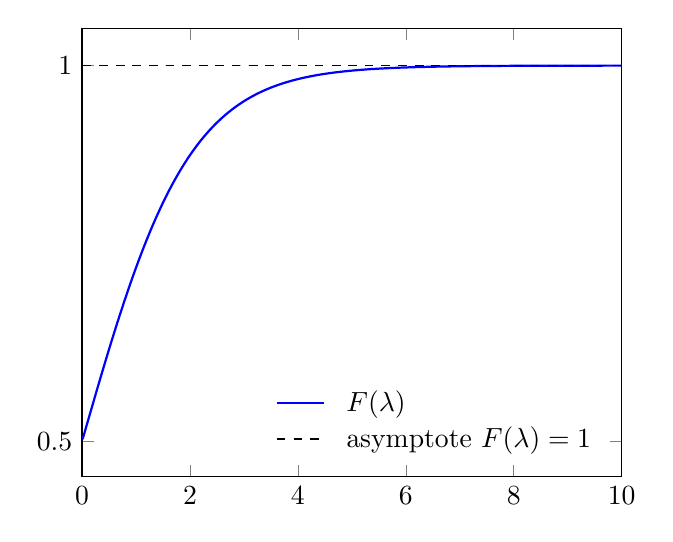
\begin{tikzpicture}
	\pgfplotsset{settings/.style={legend cell align = {left},
			legend pos =  south east,
			legend style = {draw = none}}}
	\begin{axis}[settings,xmin=0,xmax=10, ytick={0.5,1}]
	
	\addplot[domain=0.01:10, samples=500,thick,color=blue]{(exp(2*x)-exp(x))/(exp(2*x)-1)};\addlegendentry{$\;\;F(\lambda)$};
	\addplot[domain=0.01:10, samples=500,dashed]{1};\addlegendentry{\;\;asymptote $F(\lambda)=1$};
		\end{axis}
	\end{tikzpicture}\caption{Profile of the function $F(\lambda)$ for $\lambda\geq 0$.}\label{F_lambda_fig}
\end{figure}

Moreover, we claim that for all $\varepsilon>0$ there exists $\lambda^\star=\lambda^\star(\varepsilon)>0$ such that 
\begin{align}\label{F_lambda_est}
	F(\lambda) + \varepsilon F(\lambda)> 1.
\end{align}
If this is the case, multiplying both sides of \eqref{F_lambda_est} by $s\alpha^+(t)$ we immediately have 
\begin{align*}
	s\alpha^+(t)\left[1-(1+\varepsilon)F(\lambda)\right]< 0.
\end{align*}
Hence
\begin{align*}
e^{s\alpha^+(t)\left[1-(1+\varepsilon)F(\lambda)\right]}< 1
\end{align*}
and we can conclude
\begin{align*}
e^{s\alpha^+(t)} < e^{s(1+\varepsilon)F(\lambda)\alpha^+(t)} = e^{s(1+\varepsilon)\alpha^-(t)}.
\end{align*}

Therefore, it only remains to prove \eqref{F_lambda_est}. First of all, since $e^{2\lambda\norm{\eta^0}{\infty}}>1$, the inequality  may be rewritten as
\begin{align}\label{G_lambda}
	G(\lambda):=\varepsilon e^{2\lambda\norm{\eta^0}{\infty}} - (1+\varepsilon)e^{\lambda\norm{\eta^0}{\infty}} + 1> 0.
\end{align}

Moreover, \eqref{G_lambda} can be seen as a second order inequality in the variable $e^{\lambda\norm{\eta^0}{\infty}}$, whose discriminant is given by $\Delta = (1-\varepsilon)^2$. Hence, we shall distinguish between two cases:
\begin{itemize}
	\item[(i)] $\Delta = 0\Rightarrow \varepsilon=1$;
	\item[(ii)] $\Delta>0\Rightarrow \varepsilon\neq 1$.
\end{itemize}
In the case (i) we easily obtain 
\begin{align*}
	G(\lambda)=\left(e^{\lambda\norm{\eta^0}{\infty}}-1\right)^2>0
\end{align*} 
for all $\lambda>0$. In the case (ii), instead, we can readily check that the roots of $G(\lambda)=0$ are given by 
\begin{align*}
	\lambda_1:=\frac{1}{\norm{\eta^0}{\infty}}\log\left(\frac 1\varepsilon\right),\;\;\; \lambda_2:=0.
\end{align*}

Therefore, for $\varepsilon>1$ we have $\lambda_2>\lambda_1$ and, consequently, \eqref{G_lambda} holds for all $\lambda>\lambda_2$. For $0<\varepsilon<1$, instead, we have $\lambda_1>\lambda_2$ and \eqref{G_lambda} holds for all $\lambda>\lambda_1$. Summarizing, we finally have that the estimate \eqref{F_lambda_est} holds for all $\lambda>\lambda^\star(\varepsilon)$, with
\begin{align}\label{lambda_zero}
	\lambda^\star(\varepsilon):=\begin{cases}
	\D\frac{1}{\norm{\eta^0}{\infty}}\log\left(\frac 1\varepsilon\right), & 0<\varepsilon<1,
	\\
	0, & \varepsilon\geq 1.
	\end{cases}
\end{align}
\end{proof}

Proposition \ref{carleman z_prop} can now be applied to the solutions to \eqref{e11s1}, and we obtain the following Carleman estimate.

\begin{proposition}\label{carleman_phi_prop} 
Let $\varphi^T\in L^2(\Omega)$ and assume that the kernel $K$ satisfies \eqref{K_est_gen}. Then, there exist positive constants $C$, $\lambda_0(\varepsilon)$ and $\sigma_2$ such that the solution $\varphi$ to \eqref{e11s1} corresponding to the initial datum $\varphi^T$ satisfies  
\begin{align}\label{e5s2}
	\mathcal{I}(\varphi) \leq C s^3\lambda^4\intd_{\mathcal O\times(0,T)} e^{-2s\alpha}\xi^3 |\varphi|^2\,dx\,dt, 
\end{align}
for any $\lambda\geq \lambda_0$ and any $s\geq \sigma_2\left(T + T^2 + \mathcal{K}^{\frac 23}T^2\right)$.
\end{proposition}

\begin{proof}
We begin applying \eqref{carleman z} to $\varphi$, obtaining, for any $\lambda\geq C$ and any $s\geq \sigma_1\left(T + T^2\right)$ 
\begin{align}\label{carleman_prel}
	\mathcal{I}(\varphi) \leq C \left[s^3\lambda^4\intd_{\mathcal O\times(0,T)} e^{-2s\alpha}\xi^3 |\varphi|^2\,dx\,dt + \intd_Q e^{-2s\alpha}\left|\int_{\Omega} K(x,\theta,t)\varphi(\theta,t)\,d\theta\,\right|^2\,dx\,dt\right]
\end{align}

We are now going to deal with the second term on the right-hand side of the previous estimate. We have
\begin{align}\label{ker_int}
	\left|\int_\Omega K(x,\theta)\varphi(\theta,t)\,\right| & = \left|\int_{\Omega} e^{\varepsilon s\alpha(\theta,t)}K(x,\theta,t)e^{-\varepsilon s\alpha(\theta,t)}\varphi(\theta,t)\,d\theta\,\right| \notag
	\\	
	&\leq \left[\left(\int_\Omega e^{2\varepsilon s\alpha^+(t)}|K(x,\theta,t)|^2\,d\theta\right)\left(\int_\Omega e^{-2\varepsilon s\alpha(\theta,t)}|\varphi(x,\theta)|^2\,d\theta\right)\right]^{\frac 12}.
\end{align}
Moreover, by definition we have
\begin{align*}
	\alpha^+(t)=\frac{C(\Omega,\mathcal{O},\lambda)}{t(T-t)}.
\end{align*}	
Therefore,
\begin{align}\label{ker_int2}
\int_\Omega e^{2\varepsilon s\alpha^+(t)}|K(x,\theta,t)|^2\,d\theta = \int_\Omega e^{\frac{2\varepsilon sC}{t(T-t)}}|K(x,\theta,t)|^2\,d\theta = \int_\Omega e^{\frac{\mathcal{A}\varepsilon}{t(T-t)}}|K(x,\theta,t)|^2\,d\theta \leq \mathcal{K}^2,
\end{align}
where the constant $\mathcal{A}$ depends on $\Omega$, $\mathcal{O}$, $\lambda$ and $s$. Thus, from \eqref{carleman_prel}, \eqref{ker_int} and \eqref{ker_int2} we obtain 
\begin{align*}
	\mathcal{I}(\varphi) \leq C \left[s^3\lambda^4\intd_{\mathcal O\times(0,T)} e^{-2s\alpha}\xi^3 |\varphi|^2\,dx\,dt + \mathcal{K}^2\intd_Q e^{-2s\alpha(x,t)}\left(\int_{\Omega} e^{-2\varepsilon s\alpha(\theta,t)}|\varphi(\theta,t)|^2\,d\theta\,\right)\,dx\,dt\right].
\end{align*}

Let us now focus on the second term in the right-hand side of the above inequality. Using Fubini's Theorem we get
\begin{align*}
	\intd_Q e^{-2s\alpha(x,t)} & \left(\int_{\Omega} e^{-2\varepsilon s\alpha(\theta,t)}|\varphi(\theta,t)|^2\,d\theta\,\right)\,dx\,dt = \intd_Q e^{-2\varepsilon s\alpha(\theta,t)}|\varphi(\theta,t)|^2\left(\int_\Omega e^{-2s\alpha(x,t)}\,dx\right)\,d\theta\,dt.
\end{align*}
Notice that, according to \eqref{notation_alpha}, we have
\begin{align*}
	\int_\Omega e^{-2s\alpha(x,t)}\,dx \leq |\Omega| e^{-2s\alpha^-(t)},
\end{align*}
where $|\Omega|$ stands for the measure of $\Omega$. Hence, we can compute
\begin{align*}
	\intd_Q e^{-2\varepsilon s\alpha(\theta,t)}|\varphi(\theta,t)|^2\left(\int_\Omega e^{-2s\alpha(x,t)}\,dx\right)\,d\theta\,dt & \leq C \intd_Q e^{-2\varepsilon s\alpha(\theta,t)}e^{-2s\alpha^-(t)}|\varphi(\theta,t)|^2\,d\theta\,dt
	\\
	& = C \intd_Q e^{-2\varepsilon s\alpha(\theta,t)}e^{-2s(1+\varepsilon)\alpha^-(t)}e^{2s\varepsilon\alpha^-(t)}|\varphi(\theta,t)|^2\,d\theta\,dt
	\\
	& \leq C \intd_Q e^{-2s(1+\varepsilon)\alpha^-(t)}|\varphi(\theta,t)|^2\,d\theta\,dt.
\end{align*}	
Moreover, we recall that from Proposition \ref{alpha_min_max_prop} we have 
\begin{align*}
	e^{-s(1+\varepsilon)\alpha^-(t)}\leq e^{-s\alpha^+(t)},
\end{align*}
for any $\lambda >\lambda^\star(\varepsilon)$, where $\lambda^\star(\varepsilon)$ is given in \eqref{lambda_zero}. Whence, from the definitions \eqref{notation_alpha} of $\alpha^+$ and $\alpha^-$ we obtain
\begin{align*}
	\intd_Q e^{-2\varepsilon s\alpha(\theta,t)} e^{-2s(1+\varepsilon)\alpha^-(t)}  e^{2s\varepsilon\alpha^-(t)}|\varphi(\theta,t)|^2\,d\theta\,dt & \leq C \intd_Q e^{-2s\alpha^+(t)}|\varphi(\theta,t)|^2\,d\theta\,dt
	\\
	& \leq C \intd_Q e^{-2s\alpha(\theta,t)}|\varphi(\theta,t)|^2\,d\theta\,dt.
\end{align*}
Thus, we get
\begin{align*}
	\mathcal{I}(\varphi) \leq C \left[s^3\lambda^4\intd_{\mathcal O\times(0,T)} e^{-2s\alpha}\xi^3 |\varphi|^2\,dx\,dt + \mathcal{K}^2\intd_Q e^{-2s\alpha(x,t)}|\varphi(x,t)|^2\,dx\,dt\right].
\end{align*}
Recalling now the definition of $\mathcal{I}(\varphi)$, we then find the following estimate
\begin{align*}
	s\lambda^2\intd_Q e^{-2s\alpha}\xi & |\nabla \varphi|^2\,dx\,dt + s^3\lambda^4\intd_Q e^{-2s\alpha}\xi^3|\varphi|^2\,dx\,dt 
	\\
	&- \mathcal{K}^2\intd_Q e^{-2s\alpha}|\varphi|^2\,dx\,dt \leq C s^3\lambda^4\intd_{\mathcal O\times(0,T)} e^{-2s\alpha}\xi^3 |\varphi|^2\,dx\,dt.
\end{align*}
Therefore, thanks to \eqref{xi_est}, we finally obtain
\begin{align*}
	s\lambda^2\intd_Q e^{-2s\alpha}\xi |\nabla \varphi|^2\,dx\,dt + s^3\lambda^4\intd_Q e^{-2s\alpha}\xi^3|\varphi|^2\,dx\,dt \leq C s^3\lambda^4\intd_{\mathcal O\times(0,T)} e^{-2s\alpha}\xi^3 |\varphi|^2\,dx\,dt,
\end{align*}
for all $s>C\mathcal{K}^{\frac 23}T^2$ and for all $\lambda\geq\max\{C,\lambda^\star(\varepsilon)\}$. This, together with \eqref{e6s2} concludes the proof.
\end{proof}



\begin{remark}\label{rem_lambda}
	
Some comments on the above proof are in order. 	

\begin{enumerate}
	\item In the proof of Proposition \ref{carleman_phi_prop}, we used inequality \eqref{alpha_min_max} for absorbing the term including the kernel $K$ into the ones on the left-hand side of \eqref{e5s2}. Notice that the value of $\lambda^\star$ that ensures the validity of that inequality depends on $\varepsilon$ when $\varepsilon\in(0,1)$, and that ${\lim_{\varepsilon\to 0+}\lambda^\star(\varepsilon)=+\infty}$. 
	
	One may think that this is an issue when using \eqref{alpha_min_max} for proving the Carleman estimate. Nevertheless, this is not the case due to the following two facts:
	\begin{itemize}
		\item the value $\varepsilon=0$ is not allowed, and this implies that $\lambda^\star$, even if it is large, it is always finite;
		\item the inequality is true for any $s>0$. Therefore, no matter how large is $\lambda$, once this parameter has been fixed the term including the kernel can still be absorbed choosing $s=s(\lambda)$ large enough. 
	\end{itemize}
	
	\item The hypothesis \eqref{K_est_gen} plays a fundamental role in the previous proof. Notice that, according to this assumption, the kernel $K$, as a function of $t$, should behave like 
	\begin{align*}
		K(\cdot,\cdot,t)\sim e^{-\frac{\mathcal{A}(s,\lambda)\varepsilon}{t(T-t)}},
	\end{align*}
	i.e. it should decay exponentially as $t$ goes to $0^+$ and $T^-$. We stress that, even if $\mathcal{A}$ depends on $s$ and $\lambda$, from the computations that we presented above it is clear that the constant $\mathcal{K}$ is independent of these two parameters.
	
	\item  The assumption \eqref{K_est_gen} may appear as a quite strong restriction on the admissible kernels. Notwithstanding, it is instead a natural one, since the only thing that we are asking is integrability of $K$ with respect to the Carleman weight. Notice also that this decay is depending on $\varepsilon$ and, as $\varepsilon\to 0^+$, it is needed in time intervals which are shrinking more and more (see Figure \ref{kernel_fig}). Outside these intervals, instead, it is enough to consider bounded kernels, without further requirements. In other words, as $\varepsilon\to 0^+$, assumption \eqref{K_est_gen} becomes weaker, meaning that it allows more general kernels. On the other hand, due to technical reasons, we cannot take $\varepsilon=0$ (see point (1) above). 
	
	Finally, we mention that this is the minimum decay that we shall ask for the kernel. Indeed, following the proof of Proposition \ref{carleman_phi_prop} it is clear that imposing a weaker decay (e.g. polynomial) it is not sufficient to obtain the desired inequality.
	
	\begin{figure}[h]
		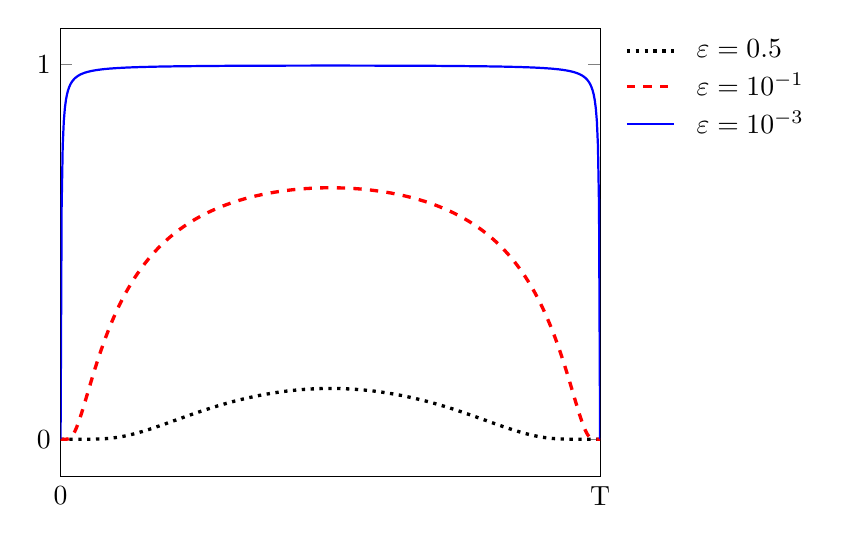
\begin{tikzpicture}
		\pgfplotsset{settings/.style={legend cell align = {left},
				legend pos = outer north east,
				legend style = {draw = none}}}
		\begin{axis}[settings,xmin=0,xmax=1,xtick={0,1},ytick={0,1},xticklabels={$0$,T}]
		
		\addplot[domain=0.0001:0.9999, samples=500, very thick,dotted]{exp(-0.5/((x*(1-x)))};\addlegendentry{$\;\;\varepsilon = 0.5$};
		\addplot[domain=0.0001:0.9999, samples=500, very thick,color=red,dashed]{exp(-0.1/((x*(1-x)))};\addlegendentry{$\;\;\varepsilon = 10^{-1}$};
		\addplot[domain=0.0001:0.9999, samples=500,thick,color=blue]{exp(-0.001/((x*(1-x)))};\addlegendentry{$\;\;\varepsilon = 10^{-3}$};
		\end{axis}
		\end{tikzpicture}\caption{Decay in the time variable of $e^{-\frac{\mathcal{A}\varepsilon}{t(T-t)}}$ for different values of $\varepsilon$. }\label{kernel_fig}
	\end{figure}
\end{enumerate}
\end{remark}

\begin{proof}[Proof of Theorem \ref{th2s1}]

First of all, from \eqref{e5s2} we clearly have
\begin{align*}
	s^3\intd_Q e^{-2s\alpha}\xi^3|\varphi|^2\,dx\,dt \leq C s^3\intd_{\mathcal O\times(0,T)} e^{-2s\alpha}\xi^3 |\varphi|^2\,dx\,dt.
\end{align*}
Moreover, due to the definition of the weight function $\alpha$ (see \eqref{weight}) we have the following two estimates:
\begin{enumerate}
	\item[1.] $s^3 e^{-2s\alpha}\xi^3 \leq Cs^3T^{-6}e^{-\frac{Cs}{T^2}}\leq C(T)$
	
	\item [2.] $s^3 e^{-2s\alpha}\xi^3 \geq Ce^{-\frac{Cs}{T^2}}$, if $t\in\Big[\frac T4,\frac 34 T\Big]$
\end{enumerate}
if we choose $s\geq CT^2$. Therefore, we obtain
\begin{align}\label{obs_prel}
	\int_{\frac T4}^{\frac 34 T}\!\!\!\int_\Omega |\varphi|^2\,dx\,dt \leq C e^{\frac {Cs}{T^2}}\intd_{\mathcal O\times(0,T)} |\varphi|^2\,dx\,dt.
\end{align}

Furthermore, due to classical energy estimates, it is easy to check that $t\mapsto \norm{\varphi(t)}{L^2(\Omega)}$ is an increasing function. Hence,
\begin{align*}
	\int_{\frac T4}^{\frac 34 T}\!\!\!\int_\Omega |\varphi(x,t)|^2\,dx\,dt \geq \int_{\frac T4}^{\frac 34 T}\!\!\!\int_\Omega |\varphi(x,0)|^2\,dx\,dt = \frac T2 \norm{\varphi(x,0)}{L^2(\Omega)}^2,
\end{align*}
and from this last estimate and \eqref{obs_prel} we finally obtain \eqref{e12s1}.
\end{proof}

Once we have the observability inequality, the control $v$ driving the solution $y$ to \eqref{e1s1} from the initial datum $y_0$ to zero can be identified as $v=\left.\varphi\right|_{\mathcal O}$, where $\varphi$ is the solution to the adjoint equation \eqref{e11s1} corresponding to an initial datum $\varphi_T\in L^2(\Omega)$ which is the unique minimizer of the functional
\begin{align}\label{functional_J}
	J\left(\varphi^T\right):= \frac 12\intd_{\mathcal O\times (0,T)} |\varphi|^2\,dxdt + \int_\Omega y_0(x)\varphi(x,0)\,dx.
\end{align}

In more detail, inequality \eqref{e12s1} ensures the coercivity of the above functional. The proof of this fact being classical, we will omit it here. 

Let us conclude this Section with a brief discussion on cost of null controllability for problem \eqref{e1s1}. We recall from \eqref{cost} that this quantity is defined as 
\begin{align*}
	\mathcal C(y_0)=\D\inf_{v\in{\mathcal O\times(0,T)}}\norm{v}{L^2(\mathcal O\times(0,T))}\,.
\end{align*}

On the other hand, it is well-known that this controllability cost may also be characterized in terms of the constant in the observability inequality \eqref{e12s1}. In more detail, we have 
\begin{align*}
	\mathcal C(y_0)=\inf_{C>0}\left\{\norm{\varphi(x,0)}{L^2(\Omega)} \leq C^2 \intd_{{ \mathcal O}\times(0,T)}|\varphi|^{2}\,dx\,dt\,\right\}.
\end{align*}
Applied to our problem, this gives the estimate
\begin{align*}
	\mathcal C(y_0)\leq\exp\left[C\left(1+\frac{1}{T}+\mathcal{K}^{\frac 23}\right)\right].
\end{align*}

In particular, as it is natural to expect for a heat-like equation, the null controllability cost blows-up as $T\to 0^+$. This means that, even if equation \eqref{e1s1} is null controllable for any time $T>0$, the cost of this process is growing exponentially as the time interval $(0,T)$ shrinks.

\section{Removing the assumption on the decay of the kernel in $t=0$}\label{decay_sec}

We are interested in showing that the assumption \eqref{K_est_gen} on the decay in time of the kernel $K$ as $t$ goes to $0^+$ and $T^-$ can be substituted by the following one, which does not requires any decay at $t=0$:
\begin{align}\label{K_est_weak}
	\mathcal{M}:=\sup_{(x,t)\in\overline{Q}}\exp\left(\frac{\mathcal{B}}{T-t}\right)\int_{\Omega} |K(x,\theta,t)|\,d\theta <+\infty.
\end{align}
Let us now introduce the new weights $\beta$ and $\gamma$ defined as

\begin{align*}
	\beta(x,t):=\frac{e^{4\lambda\norm{\eta^0}{\infty}}-e^{\lambda\left(2\norm{\eta^0}{\infty}+\eta^0(x)\right)}}{\ell(t)}, \;\;\; \gamma(x,t):=\frac{e^{\lambda\left(2\norm{\eta^0}{\infty}+\eta^0(x)\right)}}{\ell(t)},
\end{align*}
with
\begin{align*}
	\ell(t):=\begin{cases}
		\D T^2/4, & t\in\left[0,T/2\right]
		\\
		\D t(T-t), & t\in\left[T/2, T\right],
	\end{cases}
\end{align*}
and the parameters $s$ and $\lambda$ are fixed and taken as in Proposition \ref{carleman z_prop}. Then, we can state the following refined version of the Carleman inequality \eqref{carleman z}.

\begin{proposition}
There exist a positive constants $C$, depending on $T$, $s$ and $\lambda$, such that, for all $F\in L^2(Q)$ and $z_T\in L^2(\Omega)$, the solution $z$ to \eqref{syst_z} satisfies 
\begin{align}\label{carleman_z_ref}
	\norm{z(x,0)}{L^2(\Omega)}^2 + \intd_Q e^{-2s\beta}\gamma^3|z|^2\,dxdt \leq C \left[\intd_{\mathcal O\times(0,T)} e^{-2s\beta}\gamma^3 |z|^2\,dx\,dt + \intd_Q e^{-2s\beta}|F|^2\,dx\,dt\right].
\end{align}
\end{proposition}

The proof of this Proposition is standard. It combines energy estimates and the fact that $\beta\leq\alpha$ in $Q$ (see, e.g., \cite{fernandez2004local}). Furthermore, using \eqref{carleman_z_ref} and the classical approach presented in several works (\cite{fernandez2004local,fursikov1996controllability,gueye2013insensitizing,tao2016null}), it is possible to obtain the following result.

\begin{proposition}\label{control_prop_F}
Let $T>0$ and $e^{s\beta}F\in L^2(Q)$. Then, for any $y_0\in L^2(\Omega)$ there exists a control function $v\in L^2(\mathcal O\times(0,T))$ such that the associated solution to \eqref{e1s1} is in the space
\begin{align*}
	\mathcal E:=\left\{y\,:\,e^{s\beta}y\in L^2(Q)\right\}.
\end{align*}
Moreover, there exists a positive constant $C=C(T,s,\lambda)$ such that it holds the estimate
\begin{align}\label{energy_weight}
	\intd_{\mathcal O\times(0,T)} e^{2s\beta}\gamma^{-3} |v|^2\,dx\,dt + \intd_Q e^{2s\beta}|y|^2\,dx\,dt 
	 \leq C \left(\norm{y_0}{L^2(\Omega)}^2 + \norm{e^{s\beta}F}{L^2(Q)}^2\right).
\end{align}
\end{proposition} 
Notice that, $y$ being in the space $\mathcal E$, in particular we have 
\begin{align*}
	\intd_Q e^{2s\beta}|y|^2\,dx\,dt < +\infty.
\end{align*}

Since the weight $\beta$ blows-up as $t\to T^-$, the boundedness of the above integral yields $y(x,T)=0$. As a consequence, we then have the following controllability result.
\begin{proposition}
Let $T>0$ and $e^{s\beta}F\in L^2(Q)$. Then, for any $y_0\in L^2(\Omega)$ there exists a control function $v\in L^2(\mathcal O\times(0,T))$ such that the associated solution to \eqref{e1s1} satisfies $y(x,T)=0$.
\end{proposition} 
 
The above discussion can now be applied to problem \eqref{e1s1}, and we have the following result.

\begin{theorem}\label{control_thm2} 
Let $T>0$ and assume that $K$ satisfies \eqref{K_est_weak}. Then, for any $y_0\in L^2(\Omega)$, there exists a control function $v\in L^2(\mathcal O\times(0,T))$ such that the associated solution $y$ to \eqref{e1s1} satisfies $y(x,T) = 0$.	
\end{theorem}	

\begin{proof}
For $R>0$, we define 
\begin{align*}
	\mathcal E_R:=\left\{ w\in\mathcal E\,:\, \norm{e^{s\beta}w}{L^2(Q)}\leq R\right\},
\end{align*}
which is a bounded, closed and convex subset of $L^2(Q)$. For any $w\in\mathcal E_R$, let us consider the linear control problem 
\begin{align}\label{control_w}
	\begin{cases}
		\D y_t - \Delta y + \int_\Omega K(x,\theta,t)w(\theta,t)\,d\theta = v\mathbf{1}_{\mathcal O}, & (x,t)\in Q
		\\
		y = 0, & (x,t)\in\Sigma
		\\
		y(x,0) = y_0(x), & x\in\Omega.
	\end{cases}
\end{align}	
From hypothesis \eqref{K_est_weak} we have that
\begin{align*}
	\intd_Q\left(e^{s\beta}\int_\Omega K(x,\theta,t)w(\theta,t)\,d\theta\right)^2\,dxdt \leq \mathcal M^2\intd_Q e^{2s\beta}w^2e^{-2s\beta}\,dxdt \leq \mathcal M^2R^2.
\end{align*}

Therefore, from Proposition \ref{control_prop_F} we have that \eqref{control_w} is null controllable, i.e. for any $y_0\in L^2(\Omega)$, there exists a control function $v\in L^2(\mathcal O\times(0,T))$ such that the associated solution $y$ to \eqref{control_w} satisfies $y(x,T) = 0$. 

In order to conclude our proof and obtain the same controllability result for $w=y$, we shall apply Kakutani's fixed point theorem (see \cite[Theorem 2.3]{fernandez2006global}, \cite{kakutani1941generalization}). For any $w\in \mathcal E_R$, we define the multivalued map $\Lambda: \mathcal E_R\mapsto 2^{\mathcal E}$ such that
\begin{align*}
	\Lambda(w) = \left\{y\,:\,y\in\mathcal E \textrm{ and there exists } v \textrm{ such that }	\intd_{\mathcal O\times(0,T)} e^{2s\beta}\gamma^{-3} |v|^2\,dx\,dt \leq C \left(R^2 + \norm{y_0}{L^2(\Omega)}^2\right). \right\}
\end{align*} 	

It is easy to check that $\Lambda(w)$ is a nonempty, closed and convex subset of $L^2(Q)$. Moreover, by \eqref{K_est_weak} and \eqref{energy_weight} and arguing as before we have
\begin{align}\label{estimate}
	\intd_{\mathcal O\times(0,T)} e^{2s\beta}\gamma^{-3} |v|^2\,dx\,dt + \intd_Q e^{2s\beta}|y|^2\,dx\,dt 
&\leq C \left[\norm{y_0}{L^2(\Omega)}^2 + \intd_Qe^{2s\beta}\left(\int_\Omega K(x,\theta,t)y(\theta,t)\,d\theta\right)^2\,dxdt\right] \notag 
	\\
	&\leq C\left(\mathcal M^2R^2 + \norm{y_0}{L^2(\Omega)}^2\right) \leq CR^2,
\end{align}
for $R$ large enough. Hence, up to a multiplicative constant we have $\Lambda(\mathcal E_R)\subset \mathcal E_R$. 

Let $\left\{w_k\right\}$ be a sequence in $\mathcal E_R$. Then the corresponding solutions $\left\{y_k\right\}$ are bounded in $L^2(0,T;H^1_0(\Omega))\cap H^1(0,T;H^{-1}(\Omega))$ and, therefore, $\Lambda(\mathcal E_R)$ is compact in $L^2(Q)$ by Aubin-Lions' Theorem (\cite{simon1986compact}).

Notice that, for any $w\in \mathcal E_R$, we have at least one control $v$ such that the corresponding solution $y$ belongs to $\mathcal E_R$. Hence, for the sequence $\left\{w_k\right\}$ we can find a sequence of controls $\left\{v_k\right\}$ such that the corresponding solutions $\left\{y_k\right\}$ is in $L^2(Q)$. Let $w_k\to w$ in $\mathcal E_R$ and $y_k\in \Lambda(w_k)$, $y_k\to y$ in $L^2(Q)$. We want to show that $y\in\Lambda(w)$. By the regularity of the solutions and \eqref{estimate} it follows (selecting a subsequence if necessary) that
\begin{align*}
	& v_k\rightharpoonup v \textrm{ weakly in } L^2(\mathcal O\times(0,T)),
	\\
	& y_k\rightharpoonup y \textrm{ weakly in } L^2(0,T;H^1_0(\Omega))\cap H^1(0,T;H^{-1}(\Omega)),
	\\
	& y_k\to y \textrm{ strongly in } L^2(Q). 
\end{align*}
Then we obtain $y\in L^2(Q)$ and, letting $k\to +\infty$ in the system 
\begin{align*}
	\begin{cases}
		\D (y_k)_t - \Delta y_k + \int_\Omega K(x,\theta,t)w_k(\theta,t)\,d\theta = v_k\mathbf{1}_{\mathcal O}, & (x,t)\in Q
		\\
		y_k = 0, & (x,t)\in\Sigma
		\\
		y_k(x,0) = y_0(x), & x\in\Omega.
	\end{cases}
\end{align*} 
we can conclude that the couple $(y,v)$ satisfies \eqref{control_w}, i.e. $\Lambda(w) = y$. Thus the map $\Lambda$ is upper hemicontinuous.

Therefore, all the assumptions of Kakutani's fixed point theorem are fulfilled and we infer that there is at least one $y\in \mathcal E_R$ such that $y=\Lambda(y)$. By the definition of $\Lambda$, this implies that there exists at least one pair $(u,y)$ satisfying the
conditions of Theorem \ref{control_thm2}. The fact that $y(x,T) = 0$ in $\Omega$ comes from the definition of the space $\mathcal E$ and the weight function $\beta$. Hence, our assertion is proved.	
\end{proof}

\begin{remark}
As we were anticipating in Section \ref{intro_sec}, even though the approach of Theorem \ref{control_thm2} has the advantage of not requiring any decay in the kernel as $t$ goes to $0^+$, a couple of issues are worth to be commented. 
\begin{enumerate}
	\item Due to the nature of the fixed point procedure that we employed, we lose the uniqueness of the control function $v$. In particular, we are not able to identify a distinguished control with a constructive procedure. As a consequence of this fact, we also lose information about the cost of null controllability. Indeed, when a control can be computed by minimizing, for instance, the functional \eqref{functional_J}, the null controllability cost is related to the square root of the constant in the observability inequality \eqref{e12s1}. On the other hand, since the proof of Theorem \ref{control_thm2} does not requires any observability, in that case we cannot recover any explicit expression for $\mathcal C(y_0)$.
	
	\item Note that in the hypothesis \eqref{K_est_weak} we have a prescribed decay, i.e. not depending on the parameter $\varepsilon$. This arises naturally from the energy estimate \eqref{energy_weight}, which inherits the weight from the refined Carleman inequality \eqref{carleman_z_ref}.
\end{enumerate}
\end{remark}	


\section{Additional comments and open problems}\label{comments_sec}

\subsection{On the necessity of hypothesis \eqref{K_est_gen}}

As anticipated in Remark \ref{rem_lambda}, hypotheses on the kernel $K$ more general that just being bounded are necessary. Indeed, not imposing any assumption further than $\norm{K}{\infty}<+\infty$ may lead to the failure of the unique continuation of the solutions to the adjoint system. In fact, in absence of additional conditions on the kernel, it is possible to provide counterexamples where unique continuation (which is essential for obtaining controllability results) fails.

In what follows, we present one which has been proposed by P. Gerard. Let us consider the following one-dimensional situation. Let $u\in C_0^\infty(0,1)$ be a function verifying $u(x)=0$ for $x\in(a,b)\subset(0,1)$ but not identically zero on the whole interval $(0,1)$ (see Figure \ref{figure_u}). 

\begin{figure}[h]
	\pgfplotstableread{./data.org}{\datos}
	\begin{tikzpicture}
	\begin{axis}[xmin = -4, xmax = 3, ymin=-0.01,xtick={-4,-2.1,0.49,3}, ytick=\empty, xticklabels={$0$,$a$,$b$,$1$}]
	\addplot [solid,very thick, color=blue] table[x=0,y=1]{\datos};
	\end{axis}
	\end{tikzpicture}\caption{Example of a function $u(x)$ verifying: (i) $u\in C_0^\infty(0,1)$, (ii) $u(x)=0$ for $x\in(a,b)$ and (iii) $u\not\equiv 0$ in $(0,1).$}\label{figure_u}
\end{figure}	

Since $u$ is in particular a $L^2(0,1)$ function, we can write it in the form
\begin{align*}
	u(x)=\sum_{k\geq 1} c_k\phi_k(x),
\end{align*}
with $\phi_k(x)=\sqrt{2}\sin(k\pi x)$ and $c_k=\langle u,\phi_k\rangle_{L^2(0,1)}$. Moreover, for $0<\lambda<\pi$, we have 
\begin{align*}
	\sum_{k\geq 1}\left(k^2\pi^2-\lambda^2\right)c_k^2 >0
\end{align*}
and, up to a change of variables of the type $u\mapsto\sigma u$, $\sigma>0$, we can assume 
\begin{align*}
	\sum_{k\geq 1}\left(k^2\pi^2-\lambda^2\right)c_k^2 =1.
\end{align*}	
Define
\begin{align*}
	p(x) = \sum_{k\geq 1} \left(k^2\pi^2-\lambda^2\right)c_k\phi_k(x).
\end{align*}

It can be readily checked that $-u_{xx}-\lambda^2 u = p$ is verified in the sense of distributions. Hence $p\in C_0^\infty(0,1)$ with $p(x)=0$ in $(a,b)$, since $u$ has these properties. Moreover, by definition of $p$ we have
\begin{align*}
	\int_0^1 pu\,dx = 1.
\end{align*}
Therefore, $u$ satisfies the nonlocal elliptic problem
\begin{align} 
	\begin{cases}\label{nonlocal_elliptic}
		\D -u_{xx}+\int_0^1 K(x,\theta)u(\theta)\,d\theta = \lambda^2 u, & x\in(0,1) 
		\\
		u(0)=u(1)=0
	\end{cases}
\end{align}
with $K(x,\theta)=p(x)p(\theta)$. Furthermore, by assumption $u(x)=0$ for $x\in(a,b)\subset(0,1)$ but $u\not\equiv 0$ elsewhere. 

In other words, we constructed an example of a function which is solution to \eqref{nonlocal_elliptic} and does not satisfies unique continuation. In addition, this fact can be extended to the parabolic case by means of classical techniques, thus implying the failure of any controllability property for our original equation.

To avoid these kind of situations, and to ensure the validity of unique continuation properties, in some recent works the following solutions have been proposed:
\begin{itemize}
	\item analyticity assumptions on the kernel, that allow to see it as a compact perturbation of the heat operator (\cite{fernandez2016null});
	\item kernels in the form $k(x,\theta)=\alpha(x)\beta(\theta)$, with $\alpha$ not vanishing in any subinterval of $(0,1)$, which preserve the unique continuation for the solutions (\cite[Lemma 2.15]{micu2017local}).
\end{itemize}

In the present work, thanks to \eqref{K_est_gen} and by taking advantage of the weight function $\alpha$, we are able to absorb the nonlocal term in the terms on the left-hand side of \eqref{carleman_prel}, then obtaining a nice Carleman estimate for the solution to \eqref{e11s1}. This, of course, gives us the unique continuation and allow us to prove an observability inequality, therefore a controllability result.
In conclusion, from the discussion above it is clear that kernels that are merely bounded cannot be handled when dealing with controllability problems for nonlocal equations of the type of \eqref{e1s1}. Instead, some additional condition has to be imposed. In this paper, we propose to consider kernels depending also on the time variables, and to exploit the structure of the weights in the Carleman estimate. Nonetheless, we do not know whether our approach is the best possible or if, instead, sharper results can be obtained.

\subsection{Extension to semilinear problems}

The approach of Theorem \ref{control_thm} may be combined with the methodology presented in \cite{fabre1995approximate,fernandez1997null} to deduce similar controllability results for the semilinear heat equation with globally Lipschitz nonlinearity  
\begin{align}\label{heat_nl}
	\begin{cases}
		\D y_t - \Delta y + \int_\Omega K(x,\theta,t)y(\theta,t)\,d\theta = f(y) + v\mathbf{1}_{\mathcal O}, & (x,t)\in Q
		\\
		y = 0, & (x,t)\in\Sigma
		\\
		y(x,0) = y_0(x), & x\in\Omega.
	\end{cases}
\end{align}

In the same spirit, we believe that it should not be difficult to deal with modifications of problem \eqref{heat_nl} in which the nonlinearity is included in the kernel, that is, problems in the form
\begin{align*}
	\begin{cases}
		\D y_t - \Delta y + \int_\Omega K(x,\theta,t)f\big[y(\theta,t)\big]\,d\theta = v\mathbf{1}_{\mathcal O}, & (x,t)\in Q
		\\
		y = 0, & (x,t)\in\Sigma
		\\
		y(x,0) = y_0(x), & x\in\Omega.
	\end{cases}
\end{align*}

\section{Acknowledgements} 
The authors wish to thank Prof. Enrique Zuazua (Universidad Aut\'onoma de Madrid and DeustoTech) for interesting discussions on the topic of this paper. Thanks also to Cristhian Montoya (Universidad Nacional Aut\'onoma de M\'exico) for his valuable comments that helped to improve this manuscript. Finally, a special thanks goes to Prof. Patrick G\'erard (Universit\'e Paris-Sud) for suggesting the nice counterexample that helps confirming the necessity of certain hypothesis of our work.

 
\begin{thebibliography}{99}

\bibitem{fabre1995approximate} C. Fabre, J.-P. Puel and E. Zuazua. \emph{Approximate controllability of the semilinear heat equation}. Proc. Roy. Soc. Edinburgh Sec. A, 125.1 (1995), 31-61.

\bibitem{fernandez1997null} E. Fern\'andez-Cara. \emph{Null controllability of the semilinear heat equation}. ESAIM: COCV, 2 (1997), 87-103.

\bibitem{fernandez2006global} E. Fern\'andez-Cara and S. Guerrero. \emph{Global Carleman inequalities for parabolic systems and applications to controllability}. SIAM J. Control Optim. 45.4 (2006): 1395-1446.

\bibitem{fernandez2004local} E. Fern{\'a}ndez-Cara, S. Guerrero, O. Imanuvilov and J.-P. Puel. \emph{Local exact controllability of the Navier-Stokes system}. J. Math. Pures Appl., 83.12 (2004), 1501-1542.

\bibitem{fernandez2016null} E. Fern\'andez-Cara, Q. L\"u and E. Zuazua. \emph{Null controllability of linear heat and wave equations with nonlocal spatial terms}. SIAM J. Control Optim., 54.4 (2016), 2009-2019.

\bibitem{fursikov1996controllability} A. Fursikov and O. Imanuvilov. \emph{Controllability of evolution equations}. Lect. Note Series 34. Res. Inst. Math., GARC, Seoul National University (1996).

\bibitem{gueye2013insensitizing} M. Gueye. \emph{Insensitizing controls for the Navier-Stokes equations}. Ann. I.H. Poincar\'e, AN 30.5 (2013), 825-844.

\bibitem{kakutani1941generalization} S. Kakutani. \emph{A Generalization of Brouwer's fixed point Theorem}. Duke Math. J., 8.3 (1941),  457-459. 

\bibitem{lorenzi2011two} A. Lorenzi. \emph{Two severely ill-posed linear parabolic problems}. AIP Conference Proceedings, 1329.1 (2011), 150-169.

\bibitem{micu2017local} S. Micu and T. Takahashi. \emph{Local controllability to stationary trajectories of a one-dimensional simplified model arising in turbulence}. Hal preprint, Hal Id: hal-01572317 (2017).

\bibitem{montoya2017robust} C. Montoya and L. de Teresa. \emph{Robust Stackelberg controllability for the Navier-Stokes equations}. arXiv preprint arXiv:1708.04648 (2017).

\bibitem{lissy2017internal} P. Lissy and E. Zuazua. \emph{Internal controllability for parabolic systems involving analytic non-local terms}. Hal preprint, Hal Id: hal-01574999 (2017).

\bibitem{okubo2013diffusion} A. Okubo and S.A. Levin. \emph{Diffusion and ecological problems: modern perspectives}. Springer Science \& Business Media, 2013.

\bibitem{simon1986compact} J. Simon. \emph{Compact sets in the space $L^p(0,T;B)$}. Ann. Mat. Pura Appl., 146.1 (1986), 65-96. 

\bibitem{tao2016null} Q. Tao and H. Gao. \emph{On the null controllability of heat equation with memory}. J. Math. Anal. Appl., 440.1 (2016), 1-13.
\end{thebibliography}
\end{document}








